\chapter{Current system or situation \\ 
% \small{\textit{-- Author Name}}
\index{Current system or situation}
\label{Chapter::Currentsystemorsituation}} 
\section{Background, objectives, and scope \label{Section::Backgroundobjectivesandscope}}
The instore inventory management system is an essential tool for managing inventory in a retail store. The system is responsible for tracking the movement of goods, monitoring stock levels, and ensuring that the right products are available at the right time. The current manual inventory management system is time-consuming, prone to errors, and lacks real-time visibility of inventory levels. The new instore inventory management system aims to address these challenges by automating the process, providing accurate and real-time inventory information, and enabling efficient and effective management of inventory levels.
The primary objective of the instore inventory management system is to improve the accuracy, efficiency, and effectiveness of inventory management in the retail store. Specifically, the system aims to achieve the following objectives:
\begin{enumerate}    
\item Real-time inventory visibility: Provide accurate and real-time visibility of inventory levels to store managers and staff.

\item Automated inventory tracking: Automate the process of tracking inventory movement, including receiving, stocking, and selling products.

\item Efficient inventory management: Enable efficient management of inventory levels, including setting reorder points, managing stock levels, and reducing waste.

\item Improved decision-making: Provide data analytics and reporting tools to support informed decision-making related to inventory management.
\end{enumerate}
The instore inventory management system will be designed to manage inventory for a single retail store. The system will be integrated with the existing point-of-sale (POS) system to provide real-time inventory information. The system will track the movement of goods from the time they are received into the store until they are sold or removed from inventory. The system will include features for setting reorder points, generating purchase orders, and monitoring stock levels. The system will also include reporting and data analytics tools to support informed decision-making related to inventory management.

The system will be designed to be user-friendly and intuitive to use, with minimal training required for store managers and staff. The system will be scalable, allowing for the addition of new products and the expansion of the store. The system will be designed to be compatible with existing hardware and software systems in the store. Finally, the system will be secure and reliable, ensuring the confidentiality and integrity of inventory data.

\section{Operational policies and constraints \label{Section::Operationalpoliciesandconstraints}}

\textbf{Operational policies:}
\begin{enumerate}
\item Access control: Access to the instore inventory management system will be restricted to authorized personnel only. Access credentials will be assigned on a need-to-know basis.
\item Data protection: The system will store inventory data in a secure and encrypted manner. Data backups will be taken regularly to ensure data integrity and availability in case of system failure.
\item Maintenance and support: The system will be maintained and supported by trained personnel to ensure optimal performance and reliability. Maintenance schedules will be developed to minimize disruptions to store operations.
\item Training and documentation: Store managers and staff will be provided with adequate training and documentation to ensure proper use of the system. Training will be ongoing, and documentation will be updated as needed.
\item Change management: Changes to the system, including upgrades and modifications, will be managed through a formal change management process. Changes will be tested and validated before implementation.

\end{enumerate}

\noindent
\textbf{Constraints:}
\begin{enumerate}
\item Budget: The implementation of the instore inventory management system will be subject to budgetary constraints. The cost of hardware, software, and personnel will need to be within the allocated budget.

\item Integration with existing systems: The system will need to be integrated with the existing point-of-sale (POS) system, which may have limitations on compatibility.

\item Technical limitations: The system will be subject to technical limitations, such as hardware capacity and bandwidth limitations.

\item User adoption: The success of the system will depend on the adoption by store managers and staff. The system will need to be user-friendly and intuitive to ensure adoption.

\item Regulatory compliance: The system will need to comply with all relevant regulatory requirements, including data privacy and security regulations.
\end{enumerate}

\section{Description of the current system or situation \label{Section::Descriptionofthecurrentsystemorsituation}}
The current inventory management system in the retail store is a manual process that is time-consuming and prone to errors. The process involves tracking inventory movement, monitoring stock levels, and placing orders for replenishment. The system relies on physical counts, spreadsheets, and manual record-keeping to track inventory.

The process begins with the receipt of goods from suppliers. The store manager or staff checks the goods against the purchase order and records the receipt in a manual log. The goods are then moved to the storage area, and the stock level is updated manually.

When items are sold, the store manager or staff records the sale in the point-of-sale (POS) system and manually updates the inventory count. When stock levels fall below a certain threshold, the store manager or staff manually creates a purchase order to replenish the inventory.

The current system has several limitations. Firstly, the manual process is time-consuming and prone to errors, leading to inaccurate inventory counts and stockouts. Secondly, the system lacks real-time visibility of inventory levels, making it challenging to manage stock levels effectively. Finally, the manual process does not provide data analytics and reporting tools to support informed decision-making related to inventory management.\cite{OR2020}
\begin{figure}[H]
  \centering
   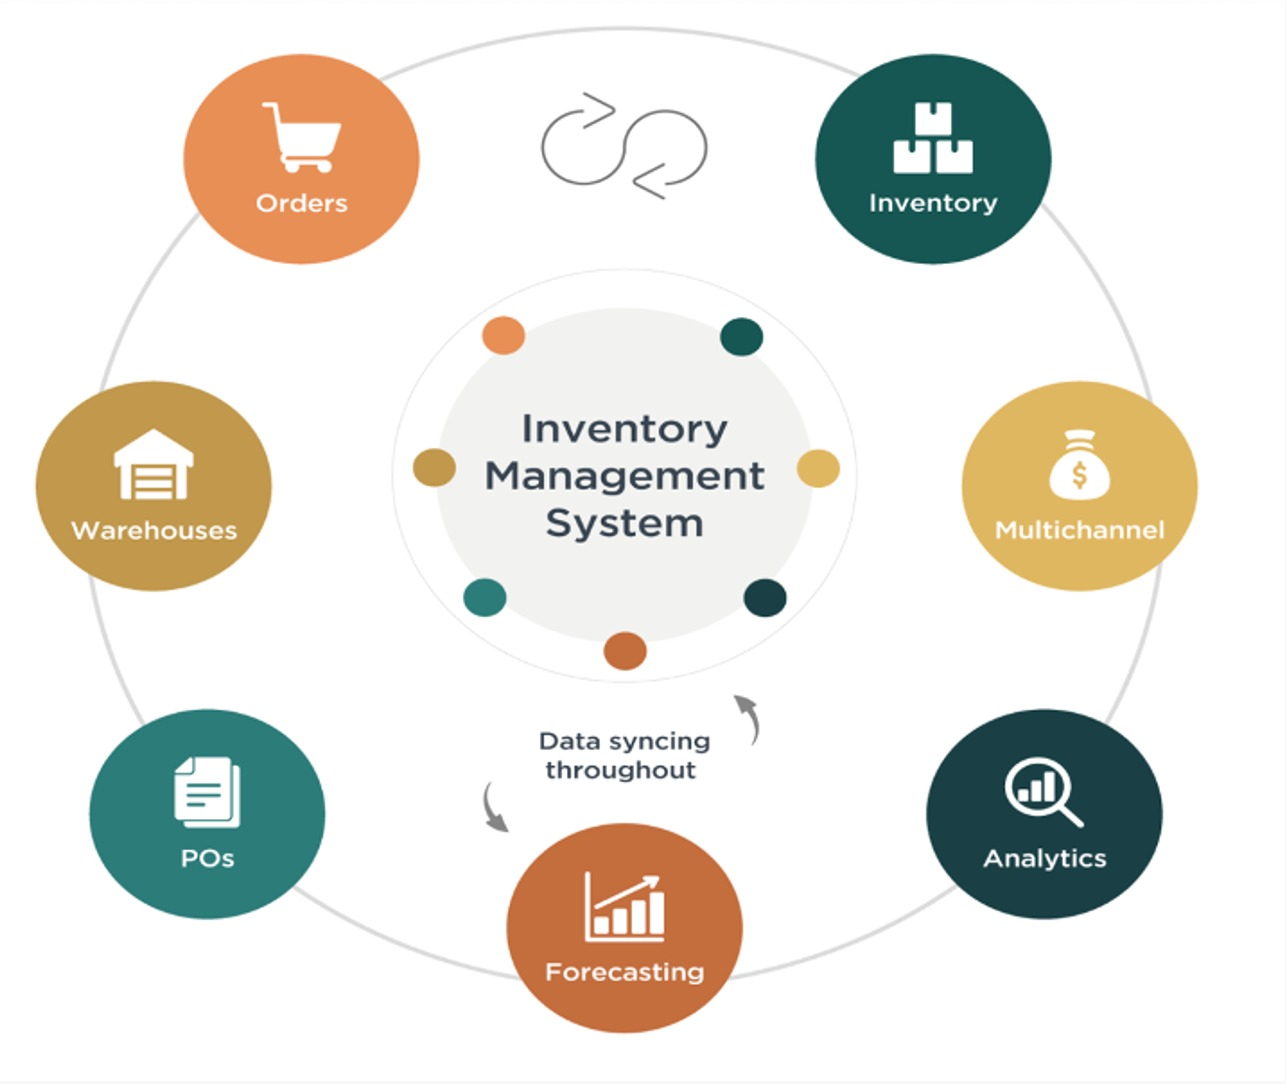
\includegraphics[width=9cm]{Figures/SpiritDiagram.jpeg}
  \caption{Overview Diagram}
\label{}
\end{figure}
\section{Modes of operation for the current system or situation \label{Section::Modesofoperationforthecurrentsystemorsituation}}
The current inventory management system in the retail store operates in the following modes:

\begin{enumerate}
    
\item Receiving mode: This mode is activated when goods are received from suppliers. The store manager or staff checks the goods against the purchase order and records the receipt in a manual log. The goods are then moved to the storage area, and the stock level is updated manually.

\item Stocking mode: This mode is activated when goods are moved from the storage area to the shelves or display areas. The store manager or staff manually updates the inventory count.

\item Selling mode: This mode is activated when items are sold to customers. The store manager or staff records the sale in the point-of-sale (POS) system and manually updates the inventory count.

\item Ordering mode: This mode is activated when stock levels fall below a certain threshold. The store manager or staff manually creates a purchase order to replenish the inventory.

\end{enumerate}

The current system operates in a sequential manner, with each mode depending on the previous mode's completion. The system lacks real-time visibility of inventory levels and does not provide automated inventory tracking or reporting tools.

\section{User classes and other involved personnel \label{Section::Userclassesandotherinvolvedpersonnel}}
The following are the user classes and other personnel involved in the instore inventory management system:

\begin{enumerate}

    \item Store manager: The store manager is responsible for managing the inventory and overseeing the instore inventory management system's operation. The store manager is responsible for setting up the system, assigning access credentials to authorized personnel, and ensuring the system's proper use.


    \item Store staff: The store staff is responsible for handling the goods, updating inventory levels, and generating reports using the instore inventory management system. The store staff will be provided with adequate training and documentation to ensure proper use of the system.

    \item IT personnel: The IT personnel will be responsible for    installing, configuring, and maintaining the hardware and software components of the system. They will also be responsible for ensuring the system's security, integrity, and availability.

    \item Suppliers: The suppliers will be involved in the system through the receipt of purchase orders generated by the system. The suppliers will need to ensure timely delivery of goods and accurate order fulfillment.

    \item Customers: The customers indirectly interact with the system by purchasing goods that are managed by the instore inventory management system. The system will ensure that the customers have access to the products they need when they need them, improving their shopping experience.
    
\end{enumerate}

The involvement of these user classes and personnel is critical to the success of the instore inventory management system, and their cooperation and support will be essential for the system's effective implementation and operation.

\section{Support environment \label{Section::Supportenvironment}}
\begin{enumerate}
    \item Help desk: A help desk will be set up to provide support and assistance to store managers and staff using the system. The help desk will be staffed by trained personnel who can provide technical assistance and troubleshooting support.

    \item Online documentation: The instore inventory management system will include online documentation that provides detailed instructions on how to use the system's features and functionality. The documentation will be regularly updated and available online for easy access.

    \item Training sessions: Store managers and staff will be provided with adequate training on the system's operation and functionality. Training sessions will be conducted both online and in-person and will be tailored to the specific needs of the user class.

    \item Maintenance and support team: A dedicated maintenance and support team will be responsible for ensuring the system's optimal performance and reliability. The team will be available to respond to system issues and perform maintenance tasks as required.

    \item Vendor support: The system vendor will provide technical support and assistance in case of system issues or malfunctions. The vendor will be responsible for ensuring that the system operates as intended and meets the user's requirements.
    
\end{enumerate}


\newpage